\begin{lemma*}[\ref{lem:center-cover}]
A parametric traversal of $P_1$ around the EB boundary is a triple cover of the locus of a Triangle Center $X_i$.
\end{lemma*}

\begin{proof}
Let $P_1(t)=\left(a \cos{t},b \sin{t}\right)$. Let $t^*$ (resp.~$t^{**})$ be the value of $t$ for which the 3-periodic orbit is an isosceles with a horizontal (resp. vertical) axis of symmetry, Figure~\ref{fig:triple-winding}, $t^*>t^{**}$. For such cases one can easily derive\footnote{It turns out $\sin{t^*}=J b$ and $\cos{t^{**}}=J a$, where $J$ is the $N=3$ Joachmisthal's constant \cite{sergei91}.}:

\begin{equation*}
\tan{t^*}=\frac{b\sqrt{2\delta-{a}^{2}+2\,{b}^{2}}}{a^{2}}, \;\;\;\tan{t^{**}}=  \frac{ \sqrt {2\,\delta-2\,{a}^{2}+{b}^{2}}}{\sqrt{3}\, a}
%\sin{t^*}=\frac{b\,\sqrt{2\delta-a^2-b^2}}{a^2-b^2}
\end{equation*}

\noindent with $\delta=\sqrt{a^4-a^2 b^2+b^4}$ as above. Referring to Figure~\ref{fig:triple-winding}:

\begin{affirmation}
\label{obs:tstar1}
A continuous counterclockwise motion of $P_1(t)$ along the intervals $[-t^*,-t^{**})$, $[-t^{**},0)$, $[0,t^{**})$, and $[t^{**},t^*)$ will each cause $X_i$ to execute a quarter turn along its locus, i.e., with $t$ varying from $-t^*$ to $t^*$, $X_i$ will execute one complete revolution on its locus\footnote{The direction of this revolution depends on $X_i$ and its not always monotonic. The observation is valid for elliptic or non-elliptic loci alike.}.
\end{affirmation}

\begin{affirmation}
\label{obs:tstar2}
A continuous counterclockwise motion of $P_1(t)$ in the $[t^*,\pi-t^{*})$ (resp.~$[\pi-t^{*},\pi+t^{*})$, and $[\pi+t^{*},2\pi-t^*)$), visits the same 3-periodics as when $t$ sweeps $[-t^*,-t^{**})$ (resp.~$[-t^{*},t^{*})$, and $[t^*,\pi-t^*)$).
\end{affirmation}

Therefore, a complete turn of $P_1(t)$ around the EB visits the 3-periodic family thrice, i.e., $X_i$ will wind thrice over its locus.
\end{proof}

\begin{figure}
    \centering
    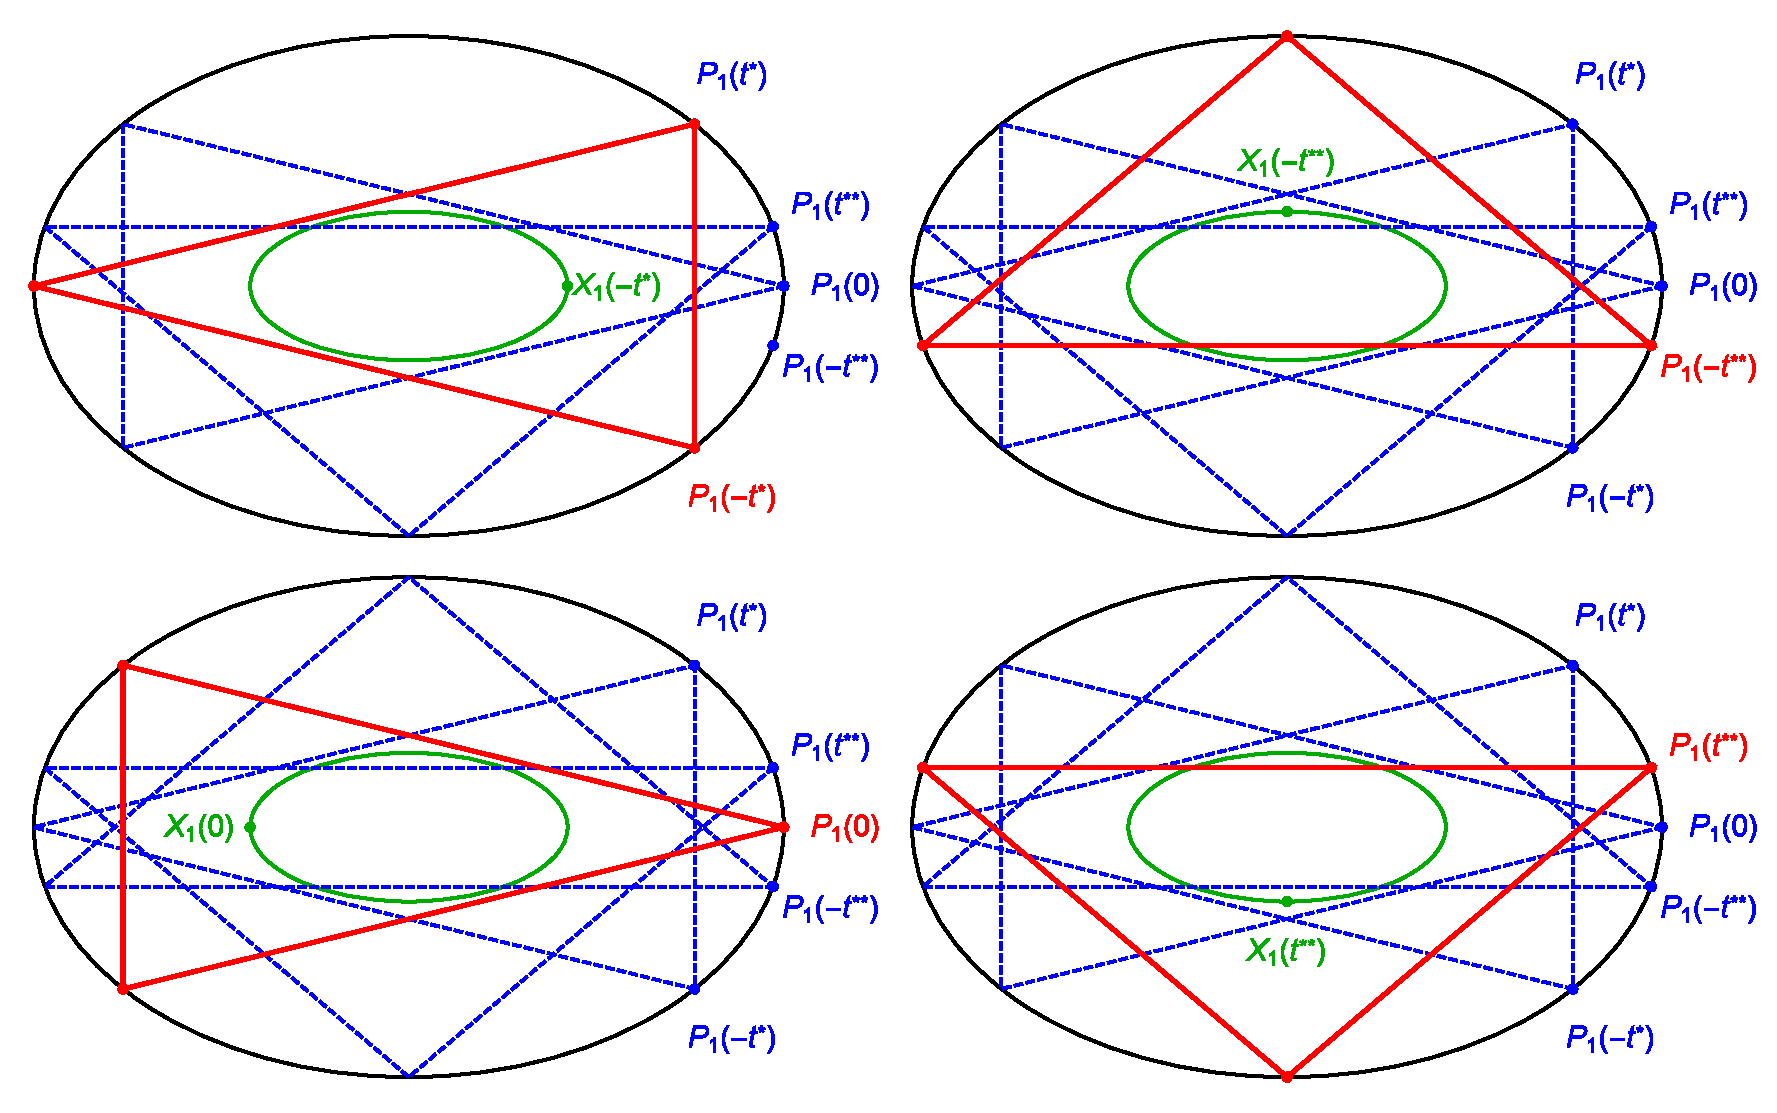
\includegraphics[width=.9\textwidth]{pics_1080_two_isosceles_tstar}
    \caption{Counterclockwise motion of $P_1(t)$, for $t=[-t^*,t^*)$ can be divided in four segments delimited by $t=(-t^*,-t^{**},0,t^{**},t^{**})$. Orbit positions for the first four are shown (red polygons) in the top-left, top-right, bot-left, and bot-right pictures. At $P_1({\pm}t^*)$ (resp.~$P_1({\pm}t^{**})$) the orbit is an isosceles triangle with a horizontal (resp.~vertical) axis of symmetry. Observations~\ref{obs:tstar1},\ref{obs:tstar2} assert that a counterclockwise motion of $P_1(t)$ along each of the four intervals causes a Triangle Center $X_i$ to execute a quarter turn along its locus (elliptic or not), and that a complete revolution of $P_1(t)$ around the EB causes $X_i$ to wind thrice on its locus. For illustration, the locus of $X_1(t)$ is shown (green) at each of the four interval endpoints.}
    \label{fig:triple-winding}
\end{figure}
Below we provide proofs of Lemmas \ref{lem:axis-of-symmetry}, \ref{lem:axisymmetric} and \ref{lem:center-cover}.
\begin{lemma*}[\ref{lem:axis-of-symmetry}]
Any Triangle Center $X_i$ of an isosceles triangle is on the axis of symmetry of said triangle.
\end{lemma*}

\begin{proof} Consider a sideways isosceles triangle with vertices $P_1=(x_1,0)$, $P_2=(-x_2,y_2)$
and $P_3= (-x_2,-y_2)$, i.e., its axis of symmetry is the $x$ axis. Let $X_i$ have Trilinears $p:q:r=h(s_1,s_2,s_3):h(s_2,s_3,s_1):h(s_3,s_1,s_2)$. Its Cartesians are given by Equation~\eqref{eqn:trilin-cartesian}. As $s_2=s_3$ and $h$ is symmetric on its last two variables $h(s_1,s_2,s_3)=h(s_1,s_3,s_2)$ it follows from equation \eqref{eqn:trilin-cartesian} that $y_i=0.$ %\textcolor{red}{ronaldo: can you provide more details.
%\textcolor{blue}{Mexi acima. Temos que melhorar os labels.}}
\end{proof}

\begin{lemma*}[\ref{lem:axisymmetric}]
If the locus of Triangle Center $X_i$ is elliptic, said ellipse must be concentric and axis-aligned with the EB.
\end{lemma*}

\begin{proof}
This follows from Lemma~\ref{lem:axisymmetric}.
\end{proof}


\begin{lemma*}[\ref{lem:center-cover}]
If the locus of $X_i$ is an ellipse, when $P_1(t)$ is at either EB vertex, its non-zero coordinate is equal to the corresponding locus semi-axis length.
\end{lemma*}

\begin{proof}
The family of 3-periodic orbits contains four isosceles triangles, Figure~\ref{fig:sideways-upright-orbit}. Parametrize $P_1(t)=(a\cos t,b\sin t)$. It follows from Lemma \ref{lem:axisymmetric} that $X_i(0)=(\pm a_i,0)$, $X_i(\pi/2)=(0,\pm b_i),$  $X_i(\pi)=(\mp a_i, 0)$ and $X_i(3\pi/2)=(0,\mp b_i)$, for some $a_i,b_i$. This ends the proof. %\textcolor{red}{ronaldo}
%\textcolor{blue}{Mexi so incluindo referencia ao lema 2 }
%Therefore, with $P_1(t)$ traveling the elliptic arc $\textrm{arc}[(a,0),(0,b)]$, $X_i(t)$ goes through one of the phases $\textrm{arc}[(\pm a_i,0),(0,\pm b_i)]$.
\end{proof}






